\section{Model}
We subdivide the classic SIRD compartments, Susceptible ($S$), Infectious ($I$), Recovered ($R$) and Deceased ($D$), with sub-compartments allowing for heterogeneous areas of residence and vaccination states as well as infections by different virus types. Individuals either live in area $A$ or area $B$. They are non-vaccinated $v_0$, vaccinated with vaccine one $v_1$ or vaccinated with vaccine two $v_2$. We introduce two virus types. A wild type $w$ that serves as baseline variant and a more infectious mutant $m$ variant.
\begin{figure}[h!]
\centering
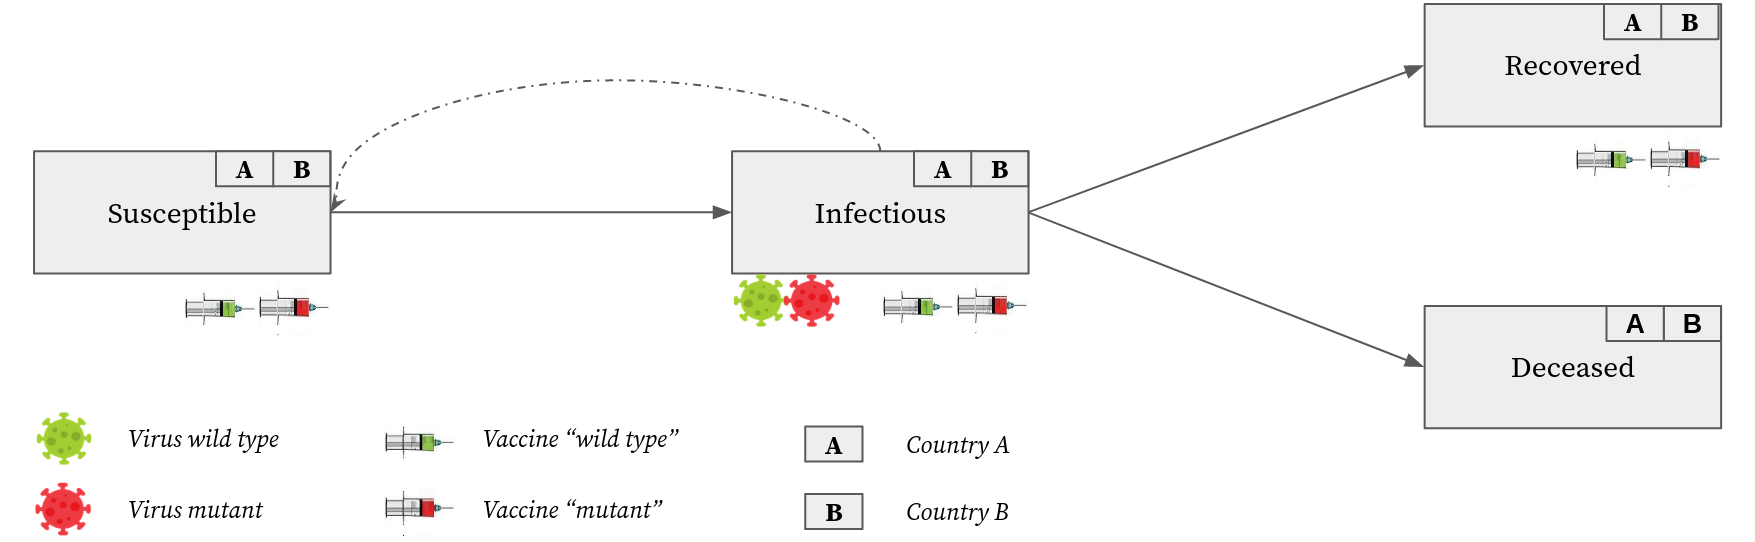
\includegraphics[scale=0.23]{images/vaccination_pp.png}
\caption{Compartments }
\end{figure}
To describe our model we follow the notation in \cite{Waites.2021} and denote every sub-group of individuals by a set $\set(F_n)$, where $F_n$ is a placeholder for features of individuals the set $\set$ is representing and $t$ denotes the time at which the set is evaluated. We illustrate this in the following by examples. Let $x_i$ for $i \in \{S, I, R, D \}$ indicate to which general compartment an individual belongs, then, $\set(x_S)$ is the set of all susceptible individuals and $\set(x_I)$ is the set of all infectious individuals in $t$. If we want to distinguish not only between general compartments but additionally between countries of residence, we use the feature $c_j$ for $j \in \{A, B\}$ to indicate that the country of residence is $j$. $\set(x_S, c_A)$ is the set of all susceptible individuals of country A and $\set(x_S, c_B)$ of country B. Note that the ordinary set operators apply, allowing us to us linkages such as $\set(x_S, c_A) \cup \set(x_S, c_B) = \set(x_S)$ or $\set(x_S) \cap \set(x_I) = \emptyset$. The cardinality $|\cdot|$ represents the respective number of individuals in a set, e.g. $|\set(x_S)|$ equals the number of all susceptible individuals. To shorthand notation, we define $\num(F_n) = |\set(F_n)|$ as the number of individuals in the compartment addressed by $(F_n)$. \\ By definition $\set() = \cup_{u \in \{ S, I, R,D\}} \set(x_u)$ is the set of all individuals. An overview of all features is given in Table \ref{tab:features}. 
\begin{table}[h!]
\centering
\caption{Notation}
\label{tab:features}
\begin{center}
\scalebox{0.8}{
\begin{tabular}{lclp{10cm}}
\hline
\multicolumn{1}{l}{Feature}&\multicolumn{1}{c}{Code}&\multicolumn{1}{c}{Indices}&\multicolumn{1}{c}{Explanation}\\
\hline
\rule{0pt}{2.6ex}General compartment & $X_h$ &  $h \in \{S, I, R, D\}$ & Individuals can either be Susceptible ($S$), Infectious ($I$), Recovered ($R$) or Deceased ($D$). \\
Country of residence & $C_j$ &  $j \in \{A, B\}$ & Individuals can either live in country A or country B.  \\
Virus Type & $V_k$ &  $k \in \{W, M\}$ & An infection can either be caused by the wild type ($W$) or the mutant ($M$) virus. This feature has to be understood, depending on $X_h$, as \textit{is} or \textit{has been} infected with type $k$. For example an individual of $\set(X_I, V_k)$ \textit{is} currently infected and an individual of $\set(X_R, V_k)$ \textit{has been} infected.\\
Vaccine Type & $U_l$ &  $l \in \{0, 1, 2\}$ & An individual can either be vaccinated with vaccine 1 or 2 or being unvaccinated ($U_0$). \\
Placeholder & $F_i$ &  $i \in \mathbb{N}$ & A placeholder that is used to address an arbitrary combination of features. $\set(F_i)$ should be read as the set of a fixed but arbitrary compartment. If we need to distinguish between two arbitrary compartments, we use $F_1$ and $F_2$.\\
\hline
\end{tabular}
}
\end{center}
%\begin{tablenotes}
%\scriptsize
%\item Note: 
%\end{tablenotes}
\end{table}

We do not incorporate reinfections. Thus, a susceptible individual cannot be associated with any virus type and therefore $\set(x_S, v_k) = \emptyset$ for all $k \in {w,m}$. Moreover, we impose a set of assumptions to our model. 
\begin{assumption}\label{ass:model}
For all $t,r \in \R_+$ and $s \in [-t, \infty)$ let
\begin{align*}
\tag{\ref{ass:model}.1} 
\label{eq:no_reinfections}
\set(x_I, v_k) \cap \mathcal{C}_{t+r}(x_S) &= \emptyset \\
\tag{\ref{ass:model}.2} 
\label{eq:no_double_vaccinations}
\set(u_1) \cap \mathcal{C}_{t+s}(u_2) &= \emptyset \\
\tag{\ref{ass:model}.3} 
\label{eq:no_cross_border_mobility}
\set(c_A) \cap \mathcal{C}_{t+s}(c_B) &= \emptyset 
\end{align*}
\end{assumption}
Assumption \ref{eq:no_reinfections} rules out reinfections. An individual that has been infected once cannot become reinfected after it had recovered. According to recent studies \textbf{cite paper} this is not true for COVID-19. However, the number of reinfected individuals is negligible and we therefore do not incorporate reinfections to keep our model parsimonious. Assumption \ref{eq:no_double_vaccinations} implies that an individual only receives one type of vaccine. Receiving one vaccination shot in our model implies that an individual is fully protected according to the vaccine properties making it unrealistic to assign a second shot to this individual. Assumption \ref{eq:no_cross_border_mobility} rules out permanent cross-country movements of individuals. According to \textbf{cite how many individuals move from one to another country} the number is negligible. We therefore decided to leave out permanent changes of residence. However, we incorporate cross-border infections via meeting rates within the mass actions.

\subsection{Mass actions and transition rules}
For a specific compartment $(F_n)$, the derivative with respect to $t$ is defined by
\begin{align*}
\der(F_n) = \lim_{r \to 0} \frac{y_{t+r}(F_n) - y_{t}(F_n)}{r}.
\end{align*}
The mass actions describe transitions from one compartment to another compartment modeled by ordinary differential equations (ODEs). We use rule-based notation to determine the system of these ODEs. A rule describes one mass action from one compartment to another compartment. We use two type of rules. The first type only has, in biological terms, one reactant and one product and the second type has two of each
\begin{align*}
	\tag{first type rule}
	\label{eq:first_type_rule}
	\num(F_1) &\xrightarrow{r_1} \num(F_2) \\
	\tag{second type rule} \label{eq:second_type_rule}
	\underbrace{\num(F_2) + \num(F_3)}_{reactants} &\xrightarrow{r_2} \underbrace{\num(F_3) + \num(F_4)}_{products}.
\end{align*}
The logic is that the individuals of the reactant compartment leave their compartment and enter a specified product compartment. This has two implications. First, the sum of the stoichiometric coefficients of the reactants must equal the sum of the stoichiometric coefficients of the products. Secondly, reactants enter the corresponding ODE negatively and products positively and mass actions are additive. Translating the system from above into ODEs leads to
\begin{align*}
	\der(F_1) &= - r_1 \cdot \num(F_1) \\
	\der(F_2) &= r_1 \cdot \num(F_1) - r_2 \cdot \num(F_2) \num(F_3) \\
	\der(F_3) &= 0 \\
	\der(F_4) &= r_2 \cdot \num(F_2) \num(F_3) .
\end{align*} 
Note that $\num(F_3)$ is reactant and product and therefore $\der(F_3) = r_2 \cdot \num(F_2) \num(F_3) - r_2 \cdot \num(F_2) \num(F_3) = 0$.
Since our model consists of many rules, we do not write down the ODE system explicitly but implicitly via the rules.
 
\subsubsection{Susceptible to Infectious}
Every infection happens between an infectious individual $i_1 \in \set(x_I)$ and a susceptible individual $i_2 \in \set(x_S)$ and leads to two infectious individuals. The rules are in form of the \ref{eq:second_type_rule}. The transition rates, which are in this case infection rates, depend on the average number of total contacts, the type of virus the infectious individual is infected with, the vaccination status of both individuals and if both individuals are from the same country
\begin{align*}
\text{infection rate} = \text{average contacts} \times \text{infectiousness} \times \text{vaccine modifier} 
\end{align*}
In the following we elaborate on how to define each component of the infection rates.\\

\textbf{Infectiousness.} Let $\alpha \in [0,1]$ be the proportion of susceptible individuals that get infected if they meet a wild type infected individual, without any vaccination, and $\eta \in (1, 1/\alpha]$ be the factor with which the mutant is more infectious than the wild type. Then $\beta = \alpha c$ is the average number of individuals infected per day by $i_1$ if $i_1 \in \set(x_I, v_w, u_0)$. If $i_1 \in \set(x_I, v_m, u_0)$ the average infected number increases to $\eta \beta$. 

\textbf{Vaccine modifier.}
To account for the influence of vaccines on vaccinated susceptible individuals, we introduce the parameters $\delta_{k,l} \in [0,1]$, where $k \in \{w, m\}$ indicates the virus type and $l \in \{ 1,2\}$ the vaccine type. If $i_2 \in \set(x_S, u_l) $ for all individuals that $i_1 \in \set(x_I, v_k)$ meets, the infection rate is multiplied by $1 - \delta_{k,l}$. $\delta_{k,l}$ can be interpreted as reduce in the probability of becoming infected while meeting an infectious individual.

Moreover, vaccinated individuals have a lower probability of transmitting the virus (\textbf{Quelle}). We account for this by introducing the parameter $\gamma \in [0,1]$ and multiplying the average number of infected individuals by $(1 - \gamma)$ if $i_1 \in \set(x_I, u_1) \cup \set(x_I, u_2)$. $\gamma$ is therefore the reduction in the probability of not transmitting the virus after being vaccinated. We assume that $\gamma$ is constant over time and across vaccines (\textbf{Quelle}). 

\textbf{Average contacts.}
Let $c \in \R_+$ be the average number of toal contacts (planned an unplanned) of one infectious individual per day. We want to distinguish between how many of the average contacts per day $c$ are within individuals from the same country and how many are within individuals from another country. We do so by defining probabilities that given a meeting occurs, it is with an individual from another country and multiply $c$ with the respective probability to obtain the average number individuals infected by one individual in a certain country. We use the relative population number of a country as baseline probability and add a penalty term for cross-border meetings. The negation operator $\neg$ is used to indicate that a certain feature applies for all but the specified compartment, e.g. $\set(\neg x_D)$ is the set of all alive individuals. In the following we establish in detail how we specify all probabilities. We first specify the (time dependent) probability that a randomly drawn living individual $i_2$ lives in country $B$ 
\begin{align*}
\prob_t\left(i_2 \in \set(\neg x_D, c_B)\right) =\num(\neg x_D, c_B) / \num(\neg x_D).
\end{align*}
Note that the probability depends on the state of the whole system $Y(t)$. To increase readability we omit conditioning on $Y(t)$ and directly define $\prob_t$ to be conditioned on the state of the system $Y(t)$.  
Second, we define the conditional probability that given $i_1$ is from country A, $i_2$ is from country B by adding a multiplicative penalty term $b(\cdot)$ reducing the probability of meeting individuals from other countries 
\begin{align*}
\prob_t(i_2 \in \set(\neg x_D, c_B) | i_1 \in \set(\neg x_D, c_A) ) = \prob_t\left(i_2 \in \set(\neg x_D, c_B)\right) \cdot b(d(A, B)),
\end{align*}
where $d(A, B)$ is a distance between country $A$ and country $B$ and $b: \R_+ \to [0,1]$, with 
$(B.1) \ \lim_{b \to \infty} = 0, (B.2) \ b(0) = 1$, and $ \ (B.3) \ b(d_1) < b(d_2)$, if $d_1 > d_2$, is a function that maps the distance to the penalty value. The distance could be interpreted as geographical distance. However, it could also serve to incorporate other factors, like favored holiday destinations, that encourage or discourage cross-border meetings.  By mapping the distance into the unit interval, we allow the probability of a cross-border meeting to be maximally as high as the relative population size. Condition $(b.1)$ ensures that countries that a very large distance only have small influences onto each other, $(b.2)$ defines a rather theoretical case where cross-border meetings are as likely as within-country meetings, and $(b.3)$ ensures that countries that have a greater distance have a smaller influence on each other.      We define all possible conditional meeting probabilities depending on the countries of residence analogously. To increase readability, we collect them in a matrix $\vect{M} \in \R^{2 \times 2}$. Let $m_{j_1,j_2}$ for $j_1, j_2 \in \{A, B\}$ be the entries of $\vect{M}$
\begin{align}
\label{eq:matrix_M}
\vect{M} &= \begin{pmatrix} 
m_{A,A} & m_{A,B} \\
m_{B,A} & m_{B,B} 
\end{pmatrix} \notag \\
&= \begin{pmatrix} 
\prob(i_1 \in \set(\neg x_D, c_A) | i_1 \in \set(\neg x_D, c_A) ) & \prob(i_1 \in \set(\neg x_D, c_A) | i_2 \in \set(\neg x_D, c_B) ) \\
\prob(i_2 \in \set(\neg x_D, c_B) | i_1 \in \set(\neg x_D, c_A) ) & \prob(i_2 \in \set(\neg x_D, c_B) | i_2 \in \set(\neg x_D, c_B) )
\end{pmatrix} \notag \\
&= \begin{pmatrix} 
1 - \num(\neg x_D, c_B) / \num(\neg x_D)   & \num(\neg x_D, c_A) / \num(\neg x_D)  \\
\num(\neg x_D, c_B) / \num(\neg x_D)  & 1 - \num(\neg x_D, c_A) / \num(\neg x_D)
\end{pmatrix} \cdot b\left(\text{d}(a_1, a_2) \right)
\end{align} 

%The negation operator $\neg$ is used to indicate that a certain feature applies for all but the specified compartment, e.g. $\set(\neg x_D)$ is the set of all alive individuals. We specify the probability of an individual $i_1 \in \set()$ to be in a particular subset by its relative frequency. For example, the (time dependent) probability that a randomly drawn living individual $i_1$ lives in country $A$ is $\prob_t\left(i_1 \in \set(\neg x_I, c_A)\right) =\num(\neg x_D, c_A) / \num(\neg x_D)$. Analogously, we can compute the probability the individual is from country A and susceptible by $\prob_t\left(i_1 \in \set(x_S, c_A)\right) = \num(x_S, c_A)/\num(\neg x_D)$. To compute the probability that the individual is susceptible, conditioned that it is from country $A$, we can use Bayes' formula 
%\begin{align}
%\prob_t\left( i_1 \in \set(x_S) |  i_1 \in \set(\neg x_D, c_A) \right)= \frac{\prob_t\left(i_1 \in  \set(x_S, c_A) \right)}{\prob_t\left(i_1 \in \set(\neg x_D, c_A)\right)} = \frac{\num(x_S, c_A)}{\num(\neg x_D, c_A)},
%\end{align}
%which yields just the proportion of susceptible individuals in country A.\\

What if we are not only interested in the fraction of $c$ that is between countries but also in the fraction of more specific compartments? As in the probability of meeting $i_2 \in \set(x_S, c_B, u_0)$ given a meeting between $i_1$ and $i_2$ occurs and $i_1 \in \set(x_I, v_w, c_A, u_0)$. What we are looking for is the conditional probability $\prob_t(i_2 \in \set(x_S, c_B, u_0)|i_1 \in \set(x_I, v_w, c_A, u_0))$. This to say, the probability that the individual that can be infected ($i_2$) is susceptible, unvaccinated and from area two given that individual $i_1$ is infected with the wild type, unvaccinated and from area one. 

We facilitate our model and assume that the vaccination status as well as the type of virus infection of individual $i_1$ are independent of the features of $i_2$. Assuming independence of the vaccination status implies that an unvaccinated individual $i_1$ does not change her contact habits, given a certain number of meetings, compared to her counterfactual vaccinated self. Note that this does not mean that we assume that vaccinated and unvaccinated individuals have the same average number of contacts since the probabilities are defined on \textit{conditioned a meeting occurs}. Differences in the average number of contacts between vaccinated and unvaccinated individuals can be incorporated implicitly via the vaccination parameter $\delta_{k,l}$. Furthermore, we assume that the probability is dependend on whether an individual is alive but not on the exact general compartment $S, I$ or $R$. Making use these assumptions, we can omit conditioning on $v_w$ and $u_0$ and change $x_I$ to $\neg x_D$ such that the exercise facilitates to defining $\prob_t(i_2 \in \set(x_S, c_B, u_0)|i_1 \in \set(\neg x_D, c_A))$. Using Bayes' formula we can rewrite this as
\begin{align}
\label{eq:cond_meeting_prob}
\prob_t(i_2 \in \set(x_S, c_B, u_0)|i_1 \in \set(\neg x_D, c_A)) &= \prob_t(i_2 \in \set(\neg x_D, c_B) | i_1 \in \set(\neg x_D, c_A) )  \notag \\
& \quad \cdot \prob_t(i_2 \in \set(x_S, u_0) | i_1 \in \set(\neg x_D, c_A), i_2 \in \set(\neg x_D, c_B) ) \notag \\
&= \prob_t(i_2 \in \set(\neg x_D, c_B) | i_1 \in \set(\neg x_D, c_A) )  \notag \\
& \quad \cdot \prob_t(i_2 \in \set(x_S, v_0)|i_2 \in \set(\neg x_D, c_B)) \notag\\
&= \prob_t(i_2 \in \set(\neg x_D, c_B) | i_1 \in \set(\neg x_D, c_A) ) \notag \\
& \quad \cdot \prob_t(i_2 \in \set(x_S, c_B, v_0))
\end{align} 
The conditional probability is therefore the product of the probability that $i_2$ is from country $B$ given that $i_1$ is from country $A$ and the probability that $i_2$ is a susceptible, unvaccinated individual from country $B$. Using equations \eqref{eq:matrix_M} and \eqref{eq:cond_meeting_prob} we obtain
\begin{align}
\label{eq:cond_prob_meeting_final}
\prob_t(i_2 \in \set(x_S, c_B, u_0)|i_1 \in \set(x_I, v_w, c_A, u_0)) = m_{B,A} \cdot \num(x_S, c_B, v_0) / \num(\neg x_D, c_B). 
\end{align}

\noindent \textbf{Infection rules.} With the derived probabilities we are able to specify the compartment specific infection rates and rules. We illustrate this by two examples. the first example deals with the compartments $\set(x_{I}, c_A, v_w, u_0)$ and $\set(x_{S}, c_B, u_0)$. By assumption, every individual $i_1 \in \set(x_{I}, c_A, v_w, u_0)$ has on average $c$ contacts per day. Equation \eqref{eq:cond_prob_meeting_final} defines the fraction of contacts which are between the two compartments of interest. Since both compartments are non-vaccinated compartments and $i_1 \in \set(v_w)$ the fraction of infectious contacts is $\alpha$. Thus, $i_1$ infects on average $\beta m_{B,A} \cdot \num(x_S, c_B, v_0) / \num(\neg x_D, c_B)$ susceptible, unvaccinated individuals from country B. This is done by $\num(x_{I}, c_A, v_w, u_0)$ unvaccinated, wild type infected individuals from country A. We can express the infection as \ref{eq:second_type_rule} rule by
\begin{align*}
\num(x_{I}, c_A, v_w, u_0) + \num(x_{S}, c_B, u_0) &\xrightarrow{ \frac{\beta \cdot m_{B,A} }{ \num(\neg x_D, c_B) }} \num(x_{I}, c_A, v_w, u_0) + \num(x_{I}, c_B, v_w, u_0).
\end{align*}

For the second example consider the compartments $\set(x_{I}, c_A, v_m, u_1)$ and $\set(x_{S}, c_B, u_2)$. We derive the rate analogously to the previous example. However, we need to account for vaccines and the more infectious mutant. Using the vaccine modifiers $\gamma$, $\delta_{m, 2}$ and the increase in infectiousness of the mutant $\eta$ yields
\begin{align*}
\num(x_{I}, c_A, v_m, u_1) + \num(x_{S}, c_B, u_2) &\xrightarrow{ \frac{\delta_{m,2} \gamma \eta \beta \cdot m_{B,A} }{ \num(\neg x_D, c_B) }} \num(x_{I}, c_A, v_m, u_1) + \num(x_{I}, c_B, v_m, u_2).
\end{align*}
To ensure readability we refrain from writing down all exact infection rules.

\subsubsection{Infectious to Recovered/Deceased}
The rules for the transitions from infectious to recovered or deceased can are for one individual independent of other individuals and therefore modeled as \ref{eq:first_type_rule}. For $\lambda \in \R_+$ we assume that on average an individual stays $1/\lambda$ days in the infectious state before it transmits either to the recovered or the deceased state. Thus, on average $\lambda$ individuals transmit out of each infectious compartment every day. We assume that a fraction $p \in [0,1]$ of unvaccinated individuals transmits to the deceased state and $(1-p)$ to the recovered state. $p$ can therefore be interpreted as the probability of dying after becoming infected. Note that $p$ does not depend on the virus type. The virus type therefore only influences the number of infections but not the probability of dying for infected individuals. \textbf{realistisch? Quelle} The corresponding rules for unvaccinated individuals are for $i \in \{A, B\}$ and $k \in \{w, m\}$
\begin{align}
    \set(x_I, c_j, v_w, u_0) &\xrightarrow{p \lambda} \set(x_D,c_j, v_w, u_0) \notag \\
    \set(x_I, c_j, v_w, u_0) &\xrightarrow{(1-p) \lambda} \set(x_R,c_j, v_w, u_0) 
\end{align}
Since vaccinations heavily reduce the probability of dying after being infected (\textbf{Quelle}), we introduce the parameters $\omega_{k,l} \in [0,1]$ for $k \in \{w, m\}$ and $l \in \{1,2\}$. We use $p \omega_{k,l}$ as new probability of dying due to being infected with virus $k$ after being vaccinated with vaccine $l$.$\omega_{k,l}$ is thus the reduction in the probability of dying. The corresponding rules for vaccinated individuals are for $i \in \{A, B\}, k \in \{w, m\}$ and $l \in \{1,2\}$
\begin{align}
    \set(x_I, c_j, v_k, u_l) &\xrightarrow{p \omega_{k,l} \lambda} \set(x_D,c_j, v_k, u_l) \notag \\
    \set(x_I, c_j, v_k, u_l) &\xrightarrow{(1-p \omega_{k,l}) \lambda} \set(x_R,c_j, v_k, u_l)
\end{align}

\subsubsection*{Vaccination}
For $j \in \{1,2\}$, $l \in \{1,2\}$
\begin{align*}
\set(x_S, v_0, a_l) &\xrightarrow{\nu_{j,l}(\cdot)} \set(x_S, v_j, a_l) \notag \\
\set(x_I, v_0, c_w, a_l) &\xrightarrow{\nu_{j,l}(\cdot)} \set(x_I, v_j, c_w, a_l) \notag \\
\set(x_R, v_0, c_w, a_l) &\xrightarrow{\nu_{j,l}(\cdot)} \set(x_R, v_j, c_w, a_l)
\end{align*}



